\documentclass[unicode,12pt]{beamer}

\usepackage{luatexja}
\renewcommand{\kanjifamilydefault}{\gtdefault}

\usetheme{metropolis}

\usepackage[backend=biber,style=ieee]{biblatex}
\addbibresource{slide.bib}
\setbeamertemplate{bibliography item}[text]

\usepackage{url}

\usepackage{graphicx}
\usepackage{listings}
\lstset{
  basicstyle=\scriptsize\ttfamily,
  identifierstyle=\scriptsize,
  ndkeywordstyle=\scriptsize,
  tabsize=4,
  frame={single},
  frameround={ffff},
  breaklines=true,
  columns=[l]{fullflexible},
  numbers=left,
  numbersep=5pt,
  numberstyle=\tiny,
  stepnumber=1,
  lineskip=-0.5ex
}
\usepackage{caption}

\captionsetup[lstlisting]{font=scriptsize}
\captionsetup[figure]{font=scriptsize}

\renewcommand{\lstlistingname}{ソースコード} % キャプション名の変更

\usepackage{hyperref}
\def\figureautorefname~#1\null{ 図~#1\null}

\usepackage{here}

\title{サンプルスライド}
\author{情報太郎}
\date{\today}

\begin{document}

\begin{frame}
  \titlepage
\end{frame}

\begin{frame}{目次}
  \tableofcontents
\end{frame}

\section{普通の文章}

\begin{frame}{普通の文章は普通に書けばいい}
これは普通の文章です。
\end{frame}

\section{コード}

\begin{frame}[fragile]{コードを書くときは\texttt{fragile}属性を指定する}
\begin{lstlisting}[language=c,caption=サンプルコード,label=code:sample]
#include <stdio.h>

int main(void)
{
    printf("hello, %s\n", "world!");
    return 0;
}
\end{lstlisting}
\end{frame}

\section{二段組}

\begin{frame}{二段組したいときは\texttt{columns}}
  \begin{columns}[t]
    \begin{column}{0.5\textwidth}
      \begin{itemize}
      \item こっちが
      \item 左
      \item \autoref{fig:sample}はこっち
      \end{itemize}
    \end{column}
    \begin{column}{0.5\textwidth}
      \begin{figure}[htbp]
        \centering
        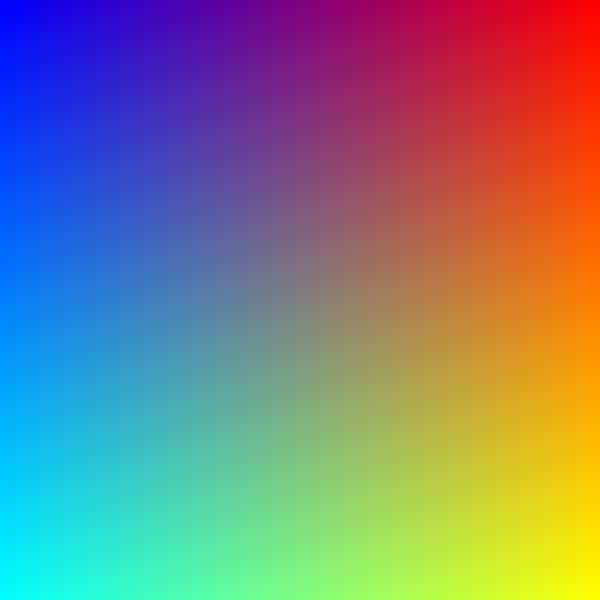
\includegraphics[width=0.45\textwidth]{sample.png}
        \caption{こっちが右}
        \label{fig:sample}
      \end{figure}
    \end{column}
  \end{columns}
\end{frame}

\begin{frame}[fragile]{二段組でもコードを書くときは\texttt{fragile}}
  \begin{columns}[t]
    \begin{column}{0.4\textwidth}
      こっちにはコードの解説を載せればいい\\
      bibしたいときは\texttt{textcite}
      \textcite{lourencco2018structured}\\
      \textcite{lourencco2016unveiling}
    \end{column}
    \begin{column}{0.6\textwidth}
      \begin{lstlisting}[language=c++,caption=C++のサンプルコード,label=code:cpp]
#include <iostream>
using namespace std;

int main() {
  cout << "hello, world!" << endl;
}
      \end{lstlisting}
    \end{column}
  \end{columns}
\end{frame}

\begin{frame}[allowframebreaks]
  \scriptsize
  \printbibliography
\end{frame}

\end{document}
